\documentclass[12pt,a4paper,latin1]{report}
\usepackage [english]{babel}

% Pour pouvoir utiliser 
%\usepackage{ucs}
\usepackage[T1]{fontenc}
\usepackage[latin1]{inputenc}
\usepackage {lmodern}
%\usepackage {picins} %image avec texte a c�t�
\usepackage{url} % Pour avoir de belles url
\usepackage {geometry}
%\usepackage{slashbox} %backslash dans tableau
%\usepackage[table]{xcolor} %couleur tableau
\usepackage{colortbl,hhline}
\usepackage{color}
\usepackage {listings} % Pour mettre du code source
\usepackage{lscape} %Pour pouvoir passer en paysage
%\usepackage {multicol} %Pour pouvoir faire plusieurs colonnes
%\usepackage{eurosym} %symbole euro
\usepackage{graphicx}
\usepackage{makeidx} %Pour cr�er un index
\usepackage {setspace} %Pour l'interligne de 1.5
%\usepackage{shorttoc} %Pour cr�er un sommaire


\usepackage[pdftex, 					% Param�trage de la navigation
bookmarks = true, 						% Signets
bookmarksnumbered = true, 				% Signets num�rot�s
pdfpagemode = UseOutlines, 					% None, UseThumbs, UseOutlines, Fullscreen
pdfstartview = Fit, 					% FitH, FitV, FitR, FitB, FitBH, FitBV, Fit
pdfpagelayout = SinglePage, 				% SinglePage, OneColumn, TwoColumnLeft, TwoColumnRight
colorlinks = false, 					% Liens en couleur
urlcolor = black, 						% Couleur des liens externes
pdfborder = {0 0 0} 					% Style de bordure : ici, rien
]{hyperref}


\hypersetup{
    unicode=false,          % non-Latin characters in Acrobat's bookmarks
    pdftoolbar=true,        % show Acrobat's toolbar?
    pdfmenubar=true,        % show Acrobat's menu?
    pdffitwindow=true,     % window fit to page when opened
    pdftitle={Rapport de projet tuteur�},    % title
    pdfauthor={Montavon Guillaume, Meilhac Benoit},     % author
    pdfsubject={\'Etude et d�veloppement avec la plate-forme Android},   % subject of the document
    pdfcreator={Montavon Guillaume, Meilhac Benoit},   % creator of the document
    pdfproducer={TexMaker (pdflatex)}, % producer of the document
    pdfnewwindow=true,      % links in new window
}


\graphicspath{{images/}}
\newcommand{\sommaire}{\shorttoc{Sommaire}{0}}
\makeindex
\definecolor{gris}{gray}{0.75}
\definecolor{orange}{rgb}{1,0.5,0}
\definecolor{vert}{rgb}{0,0.75,0}


% Pour les marges de la page
\geometry{a4paper, top=2.5cm, bottom=3.5cm, left=1.5cm, right=1.5cm, marginparwidth=1.2cm}

% Pour les entetes de page
\usepackage{fancyhdr}
\pagestyle{fancy}
\renewcommand{\sectionmark}[1]{\markboth{#1}{}} 
\renewcommand{\subsectionmark}[1]{\markright{#1}} 

\parskip=5pt %% distance entre les (paragraphe)
\sloppy %% respecter toujours la marge de droite 

% Pour les p�nalit�s :
\interfootnotelinepenalty=150 %note de bas de page
\widowpenalty=150 %% veuves et orphelines
\clubpenalty=150 

%Pour la longueur de l'indentation des paragraphes
\setlength{\parindent}{15mm}

%%%% debut macro pour enlever le nom chapitre %%%%
\makeatletter
\def\@makechapterhead#1{%
  \vspace*{50\p@}%
  {\parindent \z@ \raggedright \normalfont
    \interlinepenalty\@M
    \ifnum \c@secnumdepth >\m@ne
        \Huge\bfseries \thechapter\quad
    \fi
    \Huge \bfseries #1\par\nobreak
    \vskip 40\p@
  }}

\def\@makeschapterhead#1{%
  \vspace*{50\p@}%
  {\parindent \z@ \raggedright
    \normalfont
    \interlinepenalty\@M
    \Huge \bfseries  #1\par\nobreak
    \vskip 40\p@
  }}
\makeatother
%%%% fin macro %%%%

%red�finition maketitle pour mettre en haut de page
\makeatletter
\renewcommand{\maketitle}{%
    \vspace*{0.5cm}% ICI La taille que tu veux avant le titre
    
    \begin{center}%
    
    {\textbf{\LARGE \@title} \par}%
    \vskip 2em%
    
    {\large
     \lineskip .75em%
      \begin{tabular}[t]{c}%
        \@author
      \end{tabular}\par}%
      \vskip 1.5em%
    {\large \@date \par}%       % Set date in \large size.
    \end{center}\par
    \vskip 1.5em%
	\thispagestyle{empty}% virer num�rotation
	\setcounter{page}{0}% remettre compteur au d�but
}
\makeatother



%Couverture 

\title{
	\normalsize{D�partement Informatique\\
	Universit� de Franche-Comt�\\
	Projet tuteur�\\
	Ann�e 2010-2011}\\
	\vspace{15mm}
	\Huge{\textbf{\'Etude et d�veloppement avec la plate-forme Android}}
}

\author{MONTAVON Guillaume\\ MEILHAC Beno�t %rajouter un \\ au besoin
	\vspace{5mm}
}

\date{
	\begin{center} 
		
\includegraphics[width=14cm,height=6cm]{android.jpg}
	\end{center}
	\vspace{10mm}
	\Huge{\textbf{Rapport de projet tuteur�}}\\
	\vspace{16mm}
	\normalsize{Universit� de Franche-Comt�\\
	16 route de Gray\\
	Besan�on\\ 
	\vspace{5mm}	
	Responsables de stage :\\
        M. PIAT\\
        M. TATIBOUET
	}
}


\begin{document}

\maketitle

%\input{Remerciements}

%\sommaire
\addcontentsline{toc}{chapter}{Sommaire}
\clearpage

% Pour avoir un interligne de 1,5
\begin{onehalfspace}

\chapter{Introduction}

Mobile phone market currently knows a huge revolution with the emergence of smartphones.
This revolution was launched by Apple with its IPhone. Lots of people have been seduced by this one.
Google realized the potiential of this market and chose to get inside.
Therefore it decided to create its own Operating System (OS) for smartphones which could competed with IPhone OS\protect\footnote{IPhone Operating System} as known as IOS.
Its name is Android.

\noindent Since Android was created, it knows a very large growth.
Indeed, this OS is became the leader in sales of smartphones in the world in just two years after its placing on the market.
Due to its free access, lots of manufacturers have adopted it very quickly.
Android has a large developer community that contributes to the creation of diverse and varied applications available on Android Market, the online software store developed by Google for Android devices.

\noindent The objectives of this project were to begin with study the Android platform, which it is, what it offers to users and developers.
And in a second place, the creation of an application using the possibilities of the platform.

\noindent A first part will permit to present in details what Android is, the tools used to develop an application and the subject of this project which will present the chosen application.
Finally, a second part will describe the implemented application.

\clearpage


%\input{Presentation}

%\chapter{Context}

\section{What is Android ?}

\subsection{Presentation}

%\begin{figure}[!ht]
%    \centering
%    
\includegraphics[height=4cm]{android.png}
%    \caption{Android logo}
%
%\end{figure}
%Mettre le texte en couvrant quand possible...

\parpic[r]{
\includegraphics[height=4cm]{android.png}}

\noindent Android is an open source operating system for smartphone, PDA\protect\footnote{Personal Digital Assistant} and mobile devices. It was conceived by \textit{Android Inc.}, a startup that Google purchased in 2005. This operating system differs mainly of its competitors in that it is open, it is also used by many manufacturers and therefore smartphones on the market. Google's business model very appropriate, the adoption of Android by manufacturers has been very rapid because of the free use.

\noindent Its deployment was announced by the Open Handset Alliance (OHA) November 5 2007 and the first phone equipped end of 2008 to the United States and in the beginning of 2009 in France. Since, Android has a significant growth. It became in the beginning of 2011, first in sales of smartphones in the world.

\noindent Developer community is very active, indeed it exists more than 200 000 applications available on the Android Market, the online software store. This makes it very interesting.

\noindent More than a hundred of mobile devices are equipped of Android. Here are some examples of devices using Android :

\begin{figure}[!ht]
    \centering
    \subfloat[HTC \mbox{Desire}]{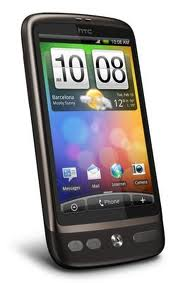
\includegraphics[scale=0.3]{htcdesire.jpg}}
    \hspace{2mm}
    \subfloat[Google Nexus One]{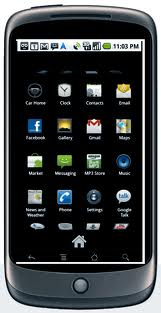
\includegraphics[scale=0.3]{googlenexusone.jpeg}}
    \hspace{2mm}
    \subfloat[Samsung Galaxy S]{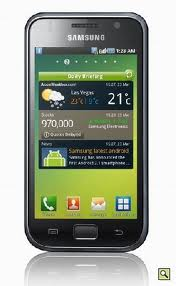
\includegraphics[scale=0.3]{samsunggalaxys.jpeg}}
    \hspace{2mm}
    \subfloat[Samsung Galaxy Tab]{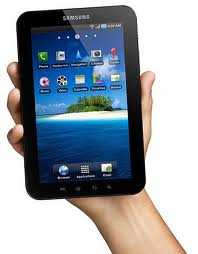
\includegraphics[scale=1]{samsunggalaxytab.jpeg}}
    \caption{Examples of devices using Android}

\end{figure}

\subsection{History}

\subsubsection{July 2005 : Purchased by Google}

\noindent A purpose of Google was to enter on market of mobile phone. That is why it purchased the small company \textit{Android Inc.} which developed applications for mobile. From that moment, Google is working on the operating system Android.

\subsubsection{November 2007 : Open Handset Alliance (OHA)}

\noindent Second key point, the creation of OHA by Google. OHA is a business alliance of many firms to develop open standards for mobile devices. There are some big names as \textit{Bouygue Telecom, Samsung or even Intel, Nvidia}.
After this alliance, the birth of the Android platform is announced.
Now, this alliance has 80 members approximately.

\subsubsection{December 2007 : Development kit}

\noindent Google publishes the first release of its SDK\protect\footnote{Software Development Kit}.

\subsubsection{September 2008 and March 2009 : First smartphone}

\noindent The first smartphone equipped of Android operation system is available for sale by \textit{T-Mobile} in September 2008 and is available in France in March 2009.

\subsubsection{October 2008 : Licensing}

\noindent Android is totally under free software/open source license and its entire source code is published.
Manufacturers can modify components and customize the system. 

\subsection{Android version}

\noindent Android has seen a number of updates since its original release. They fix bugs and add new features.\\
\noindent Generally each new version of the Android operating system is developed under a code name based on a dessert item.\\
\noindent Here are a table of Android releases :

\begin{table}[!ht]
    \begin{center}
        \begin{tabular}{|p{3.5cm}|p{5cm}|}
            \hline
                \cellcolor{gris}
                \makebox[3.5cm][c]{\textbf{Android version}}
                & 
                \cellcolor{gris}
                \makebox[5cm][c]{\textbf{Name of the version}}\\ % ligne 1
            \hline
                \textbf{1.5}
                & 
                \textbf{C}upcake\\
            \hline
                \textbf{1.6}
                & 
                \textbf{D}onut\\
            \hline
                \textbf{2.0/2.1}
                & 
                \textbf{E}clair\\
            \hline
                \textbf{2.2}
                & 
                \textbf{F}roYo <<\textit{Frozen Yogourt}>>\\
            \hline
                \cellcolor{yellow}
                \begin{minipage}{3.5cm}
                    \vspace{1mm}
                    \textbf{2.3}\\
                    \tiny{\mbox{Version} \mbox{currently} in used}
                    \vspace{1mm}

                \end{minipage}
                & 
                \cellcolor{yellow}
                \textbf{G}ingerbread\\
            \hline
                \textbf{3.0}
                &
                \textbf{H}oneycomb\\
            \hline
                \textbf{Later}
                &
                \textbf{I}ce cream sandwich\\
            \hline

        \end{tabular}
    \caption{Table of the different versions of Android}

    \end{center}

\end{table}

\noindent This is the version 2.2 which is the most used, the latest being the 2.3.

\subsection{Features}

\noindent Android has lot of functionalities, enumerate them is too long so only the most important will be presented.

\subsubsection{Extended desktop}

\noindent The desktop is extended on 3 or more parts, it depends of the manufacturer which can modify the interface. Each part is customizable by the user, it is possible to put shortcuts (to applications, folders, files, contacts, \dots) or widgets.

\subsubsection{Widgets}

\noindent Like desktop for newer operating systems, it is possible to put widget on the desktop. They can give various information and provide interaction with the system.

\subsubsection{Various sensors}

\noindent Android take in charge different sensors : accelerometers, gyroscopes, magnetometers, proximity sensors, pressure sensors or even thermometers. Lots of application use sensors, for example, Google Maps uses compass and accelerometer.

\subsubsection{Other features}

Here are some others features :
\begin{itemize}
    \item multitasking;
    \item tethering\protect\footnote{wireless connection sharing};
    \item voice based features;
    \item multi-touch;
    \item web browser;
    \item media support;
    \item new connectivity (WiFi, Bluetooth, GPS, GPRS/EDGE/3G/3G+, \dots);
    \item 3D graphics;
    \item video calling;
    \item \dots

\end{itemize}

\subsection{Android Market}

\noindent This is an online software stored developed by Google for Android devices. It is very similar to the \textit{App Store}, the online store of Apple for IPhone. This is an application preinstalled on each Android phone which one users can download applications developed by professional and individual.\\
\noindent Applications are free or pay which are sorted by category, news, \dots The research of applications is also available.

\noindent The application Android Market exists since October 2008, release of the first smartphone. There is also a website for the Android Market since February 2011 at the following address : \texttt{https://market.android.com/}.

\noindent Here are two screenshots about the Android Market :

\begin{figure}[!ht]
    \centering
    \begin{minipage}{4cm}
        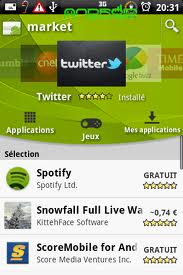
\includegraphics[width=4cm, height=7cm]{androidmarketsmartphone.jpeg}
        \caption{Application Android Market}

    \end{minipage}
%
    \hspace{0.5cm}
%
    \begin{minipage}{8cm}
        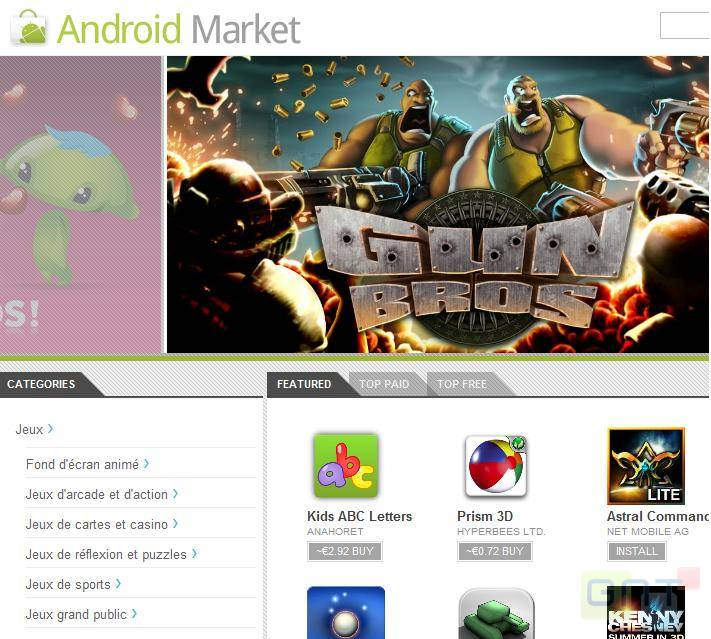
\includegraphics[width=8cm, height=7cm]{androidmarketwebsite.jpeg}
        \caption{Website Android Market}

    \end{minipage}

\end{figure}


\subsection{Android in the future}

\subsubsection{Competition}

\noindent The competition on smartphones market is hard due to its high growth. There is lot of mobile operation system, here are the four main competitor of Android.

\begin{description}
    \item[$\Rightarrow$ IOS (Apple) :] Apple famous operating system for IPhone and IPad. The first on the smartphones market. Main rival of Android.
    \item[$\Rightarrow$ BlackBerry OS (RIM) :] Research In Motion operating system for BlackBerry. It is a system in lower sales.
    \item[$\Rightarrow$ Symbian OS (Nokia) :] Symbian ltd. operating system. It equips lots of mobile phones but not really smartphones, that is why it declines.
    \item[$\Rightarrow$ Windows Phone (Microsoft) :] Microsoft operating system successor to Windows Mobile. It is a young system and not a success or a failure for now.

\end{description}

\subsubsection{View on the current market}

\noindent In only 2 years, Android became the leader in sale of smartphones in the world. Actually, there is approximately 300 000 Android smartphones sold everyday.

\noindent For the competition, IOS stagnates, BlackBerry collapses, Symbian is doomed to disappear and Windows Phone tries to find a place between Android and IOS.

\noindent Android is promised to a great future because of its exceptional growth and the fact there are more and more smartphones using this system.

\section{Presentation of the subject}

\noindent With the Android platform, the developer can have many possibilities in the creation of applications. Therefore there are so many applications available on the Android Market.

\noindent The final purpose of the project is to use more functionalities as possible in an application to get a view of what is feasible. To save development time, the software (a task manager), realized in the first semester as part of the unit value \textit{Mod�lisation, Interface utilisateur, Conception Avanc�e (MICA)}, was chosen.

\noindent So that, the project consists to :
\begin{itemize}
    \item adapt the existing application to an Android smartphone;
    \item add correctly several useful functionalities to the smartphone;
    \item have a functional application.

\end{itemize}

\section{The task manager}

\subsection{Presentation of existing}

\noindent The task manager realized as part of the unit part MICA\protect\footnote{Mod�lisation, Interface utilisateur, Conception Avanc�e} is a software for managing daily tasks that everyone should make. It is a memory aid used by everyone.

\subsubsection{Existing functionalities}

\noindent This software can realize the following actions : 
\begin{itemize}
    \item manage tags;
    \item manage tasks;
    \item sort tasks according to specific criteria;
    \item assign sub-tasks to tasks;
    \item change language via a software internationalization in English;
    \item save the tasks list.

\end{itemize}

\clearpage

\subsubsection{View of the existing}

\begin{figure}[!ht]
        \centering
        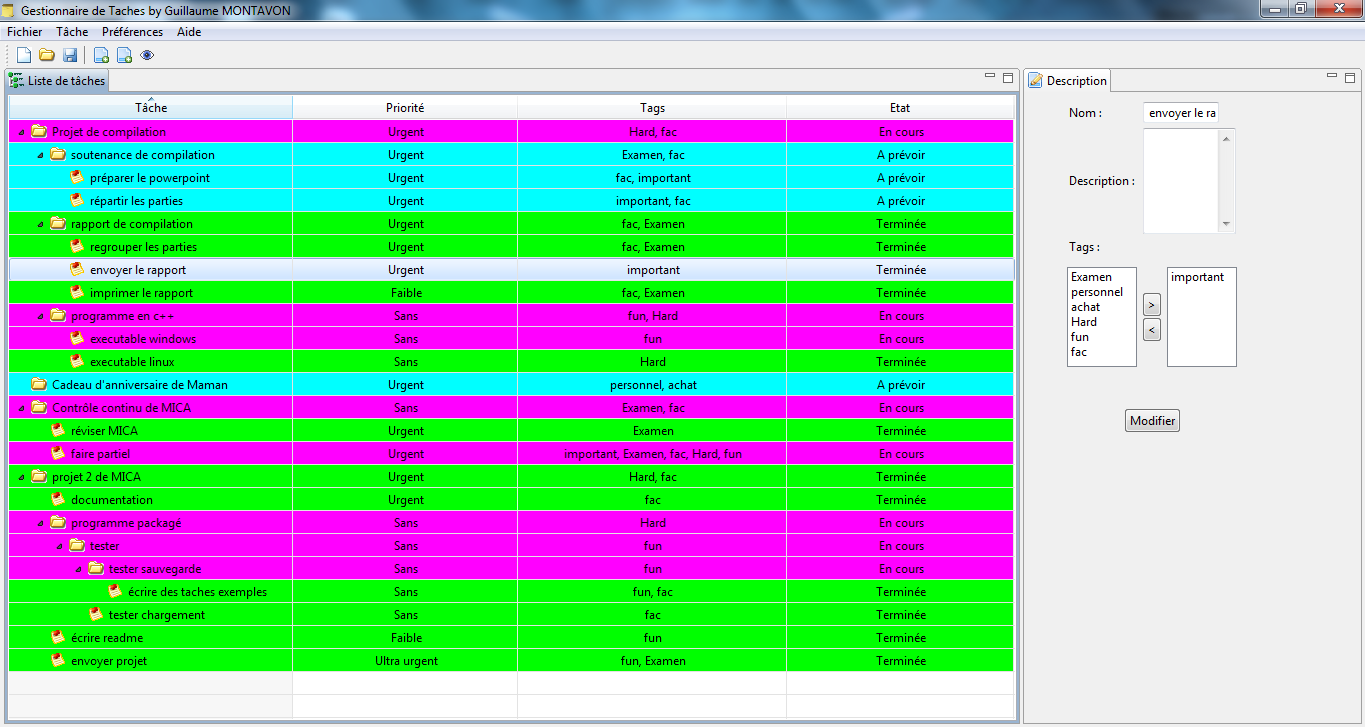
\includegraphics[width=13cm,height=8cm]{gestionnaireTacheExistantGuillaume.png}
        \caption{Example of screenshot of the existing task manager}

\end{figure}


\subsection{Presentation of the software for smartphones}

\noindent The software must be able to adapt to a smartphone while containing the functionalities listed above. That is to say, he must be able to adapt to screen size, have a simple interface and not over-elaborate, but still full. It must also include new possibilities available with Android.

\noindent Omitting the functionalities already listed in the presentation of the existing, the task manager for smartphone must be able to :
\begin{itemize}
    \item use the SQLite database available on Android smartphones;
    \item synchronize with a remote server;
    \item use the various functionalities included with Android;
    \item manage user accounts on the server.

\end{itemize}

\section{Specifications}

\subsection{Application design}

\noindent The application can be divided into different main parts.
One general part that reflects the objectives of the first software task manager.
One part concerning the storage of information on the smartphone.
And a last part to manage the remote server.

\noindent The general objectives of the application are :
\begin{itemize}
    \item manage the application with tasks and tags (added, remove, modification, sorting);
    \item a graphical interface fluid and pleasant to use while still powerful and complete;
    \item internationalization of the application in English;
    \item manage the application preferences.

\end{itemize}

\vspace{0.5cm}

\noindent Concerning the database :
\begin{itemize}
    \item creation of a coherent basis to manage all the data of the application;
    \item storing, modifying and deleting data.

\end{itemize}

\vspace{0.5cm}

\noindent Concerning the synchronization with the remote server :
\begin{itemize}
    \item creation of a database more evolved than the smartphone;
    \item sending and receiving data with their storage, modification and deleting;
    \item manage users;
    \item implementation of various methods of synchronization :
    \begin{itemize}
        \item overwrite data from the smartphone replaced by those of the server;
        \item overwrite data from the server replaced by those of the smartphone;
        \item combine data of the server and the smartphone.

    \end{itemize}
    \item manage a proxy server.

\end{itemize}

\subsection{Technical constraints}

\noindent Developing an application with Android imposes some constraints to have a result.

\subsubsection{Development tools}

\noindent Several tools are available to easily develop with Android :
\begin{itemize}
    \item Google Android SDK\protect\footnote{Software Development Kit} which contains an emulator of smartphone;
    \item eclipse IDE\protect\footnote{Integrated Development Environment} to develop in Java;
    \item Android plugin ADT which one can to use the emulator with eclipse.

\end{itemize}


\subsubsection{Web server}

A web server was set up to test remote synchronization. This server is hosted by \textit{OLikeOpen} (web host which offer his services for free) and has a MySQL database and PHP tools for communicating with it.

\subsubsection{Miscellaneous}

There are lot of version of Android and they evolve everyday, so this is why the development was completed and tested on 2.2 version (\textit{FroYo}).
However, an emulator is not sufficient to verify the correct running of the application, a smartphone that has the correct version of Android was necessary to validate the tests.

\subsection{Temporal constraints}

The first part of the project consists to the study of the Android platform, so the development time of the application depends of time to get one's feet wet with the tools proposed by Android.
The rest of the time is a full development of the task manager.

\clearpage


%\chapter{Cahier des charges}

\section{Conception de l'application}

\noindent Les objectifs généraux de l'application sont :
\begin{itemize}

\end{itemize}




%\input{Mise}

%\input{Bilan}

%\chapter{Conclusion}

\vspace{2cm}

\noindent The first large part of this project has given an overview on Android platform. It revealed, among other things, how does Android work, possibilities but also limits. What was important for the continuation of the project, concerning the programming, it was the discovery of the tools necessary to develop. The second part could be started serenely.

\noindent In this second part, once the choice of the application made, it was necessary to do a short study on the functionalities, improvements and customizations. The task manager is now functional, it enables management of tasks and tags on a remote server to a specific user.

\noindent To conclude, the study of the platform has acquired new knowledges, to know more details about Android and what goes around. This study gives an overview of the product.
After that, the development of a compatible application for Android smartphones revealed in greater depth Android, its functioning system, the limitations and the possibilities.
Finally, work on the Android platform was full of knowledges. This platform, in constant evolution, continue to seduce more and more people by adapting easily on their needs.


\clearpage


%% Pour finir l'interligne de 1,5
\end{onehalfspace}

\clearpage
\newpage

%\chapter{Glossary}

\vspace{2cm}

\textbf{1 : } ...

\vspace{3mm}

\textbf{2 : } ...

\clearpage


%%----------------------------------------
%% Pour la bibliographie
%%----------------------------------------
%% Citer tous les ouvrages/r�f�rences
\nocite{*}
%% Trier par ordre d'apparition
\bibliographystyle{unsrt}
%% Pour le style de la biblio
\bibliographystyle{plain}
%% Ecrire la biblio ici
%\bibliography{Bibliographie}
\addcontentsline{toc}{chapter}{Bibliographie}

\clearpage
\newpage

%\input{Annexe}

\printindex

\appendix

\listoftables
\addcontentsline{toc}{chapter}{Liste des tableaux}
\clearpage

\listoffigures
\addcontentsline{toc}{chapter}{Table des figures}
\clearpage

\tableofcontents
\addcontentsline{toc}{chapter}{Table des mati�res}

\clearpage

%\input{Couv}

\end{document}
